%%%%%%%%%%%%%%%%%%%%%%%%%%%%%%%%%%%%%%%%%
% University/School Laboratory Report
% LaTeX Template
% Version 3.1 (25/3/14)
%
% This template has been downloaded from:
% http://www.LaTeXTemplates.com
%
% Original author:
% Linux and Unix Users Group at Virginia Tech Wiki 
% (https://vtluug.org/wiki/Example_LaTeX_chem_lab_report)
%
% License:
% CC BY-NC-SA 3.0 (http://creativecommons.org/licenses/by-nc-sa/3.0/)
%
%%%%%%%%%%%%%%%%%%%%%%%%%%%%%%%%%%%%%%%%%

%----------------------------------------------------------------------------------------
%	PACKAGES AND DOCUMENT CONFIGURATIONS
%----------------------------------------------------------------------------------------

\documentclass{article}

\usepackage[a4paper, total={6in, 8in}]{geometry}
\usepackage[version=3]{mhchem} % Package for chemical equation typesetting
\usepackage{siunitx} % Provides the \SI{}{} and \si{} command for typesetting SI units
\usepackage{graphicx} % Required for the inclusion of images
\usepackage{natbib} % Required to change bibliography style to APA
\usepackage{amsmath} % Required for some math elements 
\usepackage{enumerate} % Required for the enumerate function
\usepackage[americanvoltages,siunitx]{circuitikz} % Required for the drawing of circuit diagrams
\usepackage{caption}
\usepackage{graphicx}
\usepackage{subcaption}
\usepackage{xfrac}
\usepackage{float}
\usepackage{enumitem}
\usepackage{epstopdf}
\usepackage{booktabs}
\usepackage[]{mcode}
\usepackage{tikz}
\usetikzlibrary{shapes,arrows}
\usepackage{verbatim}
\usepackage{amssymb}
\usepackage{cprotect}

\setlength\parindent{0pt} % Removes all indentation from paragraphs

\renewcommand{\labelenumi}{\alph{enumi}.} % Make numbering in the enumerate environment by letter rather than number (e.g. section 6)

\graphicspath{{../Images/}}

%\usepackage{times} % Uncomment to use the Times New Roman font

%----------------------------------------------------------------------------------------
%	DOCUMENT INFORMATION
%----------------------------------------------------------------------------------------

\title{Digital Signal Processing \\ Tutorial 5 \\ ENG421} % Title

\author{Shane \textsc{Reynolds}} % Author name

\date{\today} % Date for the report

\begin{document}

\maketitle % Insert the title, author and date

\begin{center}
\begin{tabular}{l r}
Date Performed: & May 12, 2017 \\ % Date the experiment was performed
Instructor: & Friso DeBoer % Instructor/supervisor
\end{tabular}
\end{center}

\tableofcontents
\newpage
% If you wish to include an abstract, uncomment the lines below
% \begin{abstract}
% Abstract text
% \end{abstract}

%----------------------------------------------------------------------------------------
%	SECTION 1
%----------------------------------------------------------------------------------------

\section{Overview}
The primary objective of this laboratory is two fold:
\begin{enumerate}[label=\roman*]
	\item Investigate dual tone signal generation and detection used in telephony operation using FIR filters and frequency detection algorithms.\\
	\item Investigate amplitude modulation using a carrier signal, and subsequent demodulation. Further, reconstruct signals by performing additional modulation and filtering using a first order digital notch filter.
\end{enumerate}

%----------------------------------------------------------------------------------------
%	SECTION 2
%----------------------------------------------------------------------------------------

\section{Background and Results}
The laboratory session was broken down into two principal sections: dual tone signal generation and detection, and amplitude modulation. This section of the report will discuss the background and results of each component of the practical in turn.

\subsection{Background: Telephone Touch Tone Dialling}
Signals are used in touch tone telephones to indicate which key is being pressed. Each key could have been assigned a single distinct frequency which is not a multiple of any other frequencies, however, this would have added extra cost to the electronic components used to generate each of the 12 frequencies. A more efficient way to achieve the same result is two use a total of 7 unique frequencies, and assign each key two of these frequencies. The total number of unique combinations that we can be achieved with this method is 21 so there is some redundancy in the system, however, a stark improvement over individualised frequencies. The frequency matrix for each of the keys can be seen below in Table 1.

\begin{figure}[H]
	\centering
	\begin{tabular}{|c|c|c|c| }
		\hline
		FREQS		&	1206 (Hz)	&	1336 (Hz)	&	1447 (Hz)\\
		\hline
		697 (Hz)	&	1			&	2			&	3\\
		\hline
		770 (Hz)	&	4			&	5			&	6\\
		\hline
		852 (Hz)	&	7			&	8			&	9\\
		\hline
		941 (Hz)	&	*			&	0			&	\#\\
		\hline
	\end{tabular}
	\caption{DTMF encoding table for Touch Tone dialling. when any key is pressed the tones of the corresponding column and row are generated.}
\end{figure}
 
Signal generation of the two tone signals is straightforward. Two discrete time signals are generated at each of the corresponding frequencies for a single key press and the signals are superimposed. An illustrative example of this would be the generated signal for key 1, which would be:
\begin{align*}
	x[n] = \cos(2 \pi \cdot 697 \cdot T_s \cdot n) + \cos(2 \pi \cdot 1206 \cdot T_s \cdot n)
\end{align*}

The end of a single key press is padded with a small gap in which no signal is sent - this makes it easy to demarcate the individual key presses for some given signal which is comprised of many key presses. The received signal undergoes several steps in order to decode it

\subsection{Results: Telephone Touch Tone Dialling}
\subsubsection{DTMF Dial Function}
In order to generate a signal given a set of key presses a function \verb|dtmfdial| was implemented in MATLAB, which can be seen in Appendix A. the function takes and input vector of numbers which ranges from 1 to 12. The numbers 10, 11 and 12 were used to represent *, 0, and \#, respectively. The output of the function is a vector of the summed discrete signals for each of the two frequencies corresponding to the key pressed. As previously mentioned, to demarcated the end of a key press, a signal of 0 is appended to the end of each signal for a duration of 0.1 seconds. Figure 2 shows a spectrogram for each of the 12 key presses.

\begin{figure}[H]
	\centering
	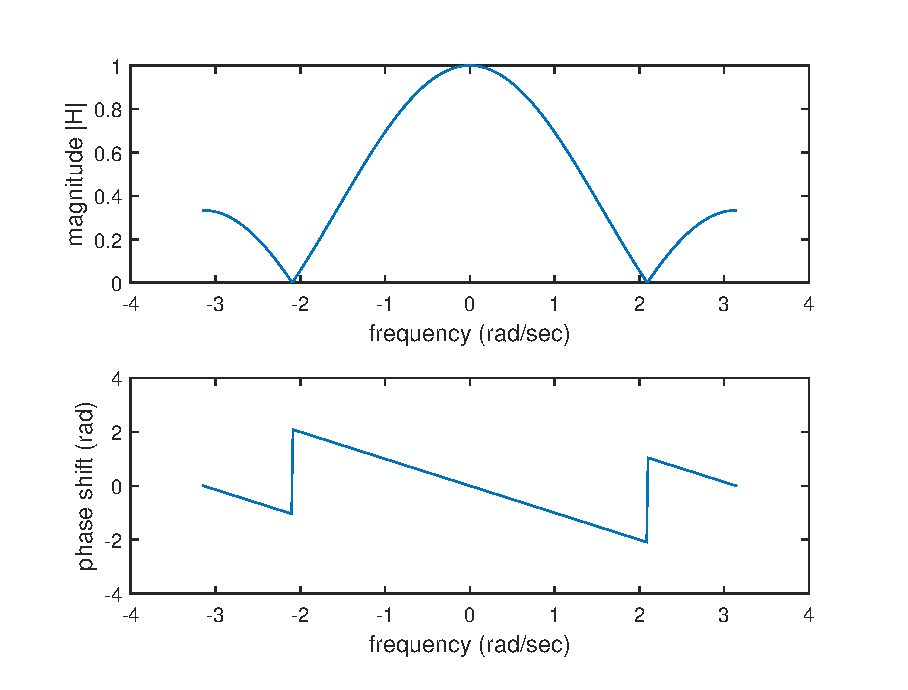
\includegraphics[scale=0.8]{fig1.eps}
	\caption{Spectrogram of the frequencies generated by each of the key presses. The dark bands represent the frequencies for each of the signals. Each band represents a key press from 1 through 12.}
\end{figure}

\subsubsection{DTMF Decoding: Filter Design}
The sent signal is received as it was originally sent, assuming a perfect communication channel. Typically, in the real world, there would be some noise introduced during the transmission of the signal and would have to be cleaned up using a high frequency filter, or a differencing output. In order to check for the presence of a frequency in a signal, a simple bandpass filter needs to be implemented for each of the 7 frequencies present in the key matrix shown in Figure 1. The filter used in this instance is of the form:
\begin{align}
	h[n] = \frac{2}{L} \cdot \cos \bigg(\frac{2 \pi f_b n}{f_s}\bigg), \quad 0 \leq n \leq L
\end{align}

A MATLAB script, shown in Appendix B, demonstrates implementation of the filter shown in (1). Figure 3 shows the filter coefficients from a filter with $f_b = 770 \si{\hertz}$ in the upper plot, and the frequency $f_b = 1336 \si{\hertz}$ in the lower plot. 

\begin{figure}[H]
	\centering
	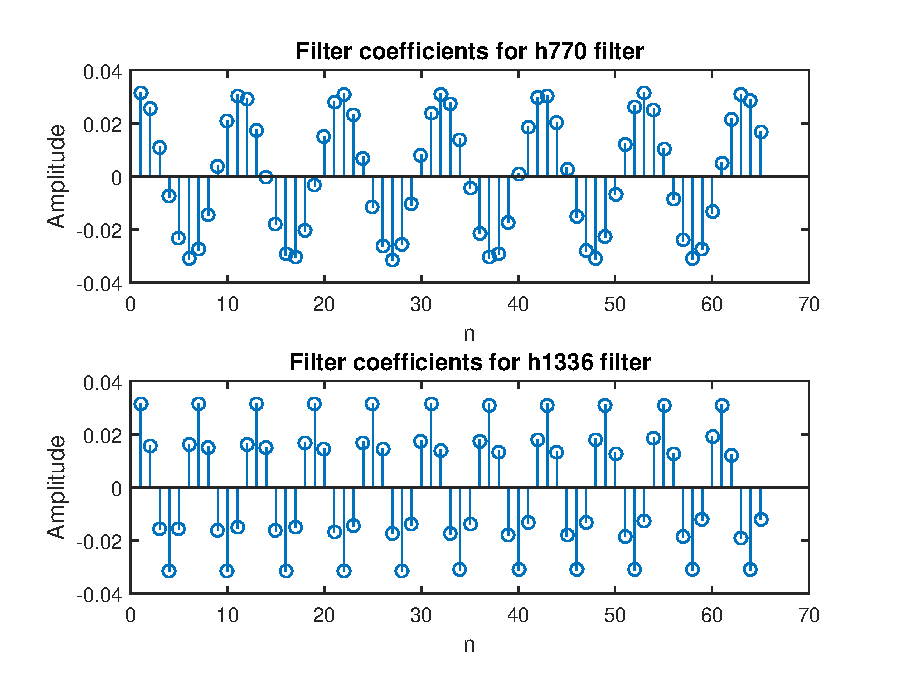
\includegraphics[scale=0.55]{fig2}
	\caption{Plots of the filter coefficients. The bandpass filter for 770 $\si{\hertz}$ is in the top plot and the bandpass filter for the 1336 $\si{\hertz}$ is in the bottom plot}
\end{figure}

The frequency response of the filter for 770 $\si{\hertz}$ is shown in Figure 4 - here it can be seen that the main lobe is centred over the desired frequency 770 $\si{\hertz}$. Similarly, Figure 5 shows the frequency response for the filter for 1336 $\si{\hertz}$, with the main lobe centred around 1336 $\si{\hertz}$.

\begin{figure}[H]
	\begin{minipage}[t]{0.5\linewidth}
		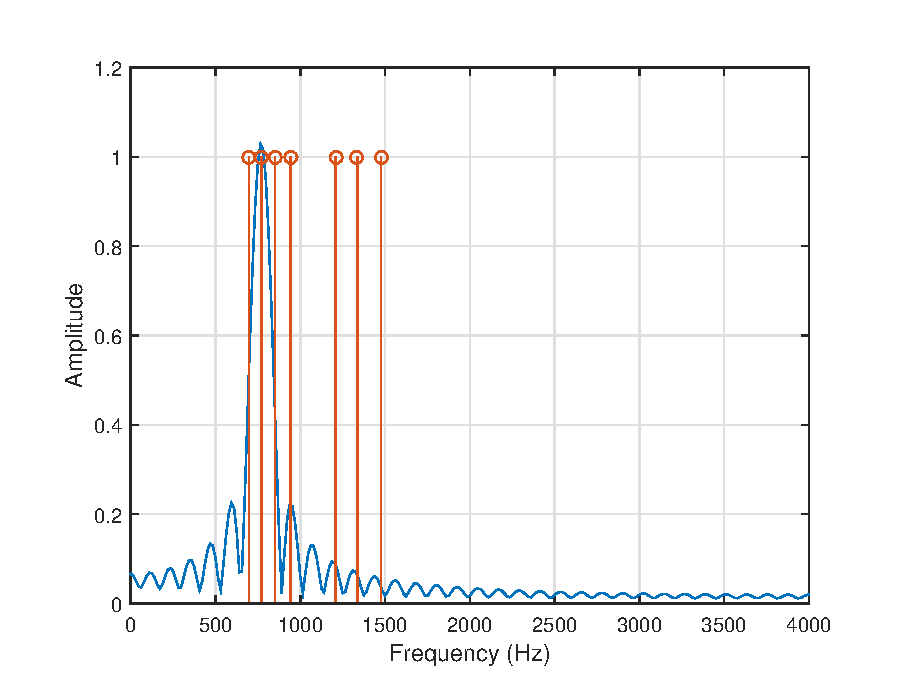
\includegraphics[scale=0.5]{fig3}
		\caption{Amplitude of the frequency response for the 770 $\si{\hertz}$ filter. The frequencies 697$\si{\hertz}$, 770$\si{\hertz}$, 852$\si{\hertz}$, 941$\si{\hertz}$, 1209$\si{\hertz}$, 1336$\si{\hertz}$, 1477$\si{\hertz}$ which represent the 7 distinct frequencies for the keying matrix have also been plotted.}
	\end{minipage}
	\hspace{0.5cm}
	\begin{minipage}[t]{0.5\linewidth}
		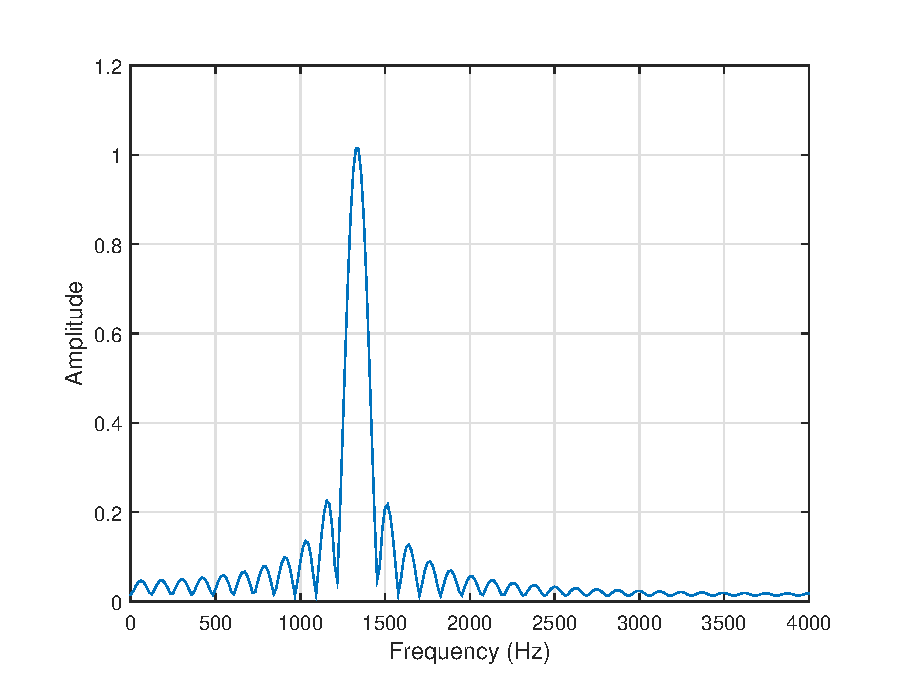
\includegraphics[scale=0.5]{fig4}
		\caption{Amplitude of the frequency\\ response for the 1336 $\si{\hertz}$ filter.}
	\end{minipage}
\end{figure}

Finding the output from a filter in the frequency domain from some given input signal $X(j \omega)$ is relatively straight forward - the frequency response, $H(j \omega)$, is multiplied by the input signal $X(j \omega)$:
\begin{align}
Y(j \omega) = H(j \omega) \cdot X(j \omega)
\end{align}

Equation (2) yields some insight in how the filter works, when considered along side the frequency response shown in Figure 4 and 5. The target frequency which is to be \textit{passed} has the signal at that frequency multiplied by 1, and the remainder of the frequencies are attenuated due to much lower amplitudes in the frequency response for the filter.

\subsubsection{DTMF Decoding: A Scoring Function}
The received signal needs to be tested to see which key was pressed, the two frequencies of the dual tone key need to be determined. The received signal is passed through a filter for a some target frequency and then tested heuristically to determine if the signal was composed of the target frequency. The heuristic is implemented in the scoring function called \verb|dtmfscor| shown in Appendix C. The last line of the code in the function is given by:
\begin{center}
	\verb|ss = (mean(conv(xx,hh).^2) > mean(xx.^2)/5)|
\end{center}

This is the decision making part of the function. The output signal after being passed through the filter, using the convolution, is squared, and the average is found. This takes the signal and makes any elements which have been attenuated small, due to the squaring operation. This result compared logically to the average of the signal squared, which is then scaled by 0.2. If the average output from the filter is greater than the average of the squared signal with scaling factor, then the function returns a true, indicating that the frequency is present at a material level. A point worth noting about the heuristic is that the scaling value of 0.2 is arbitrary and can be changed depending on the required sensitivity of the detection required.
 
\subsubsection{DTMF Decoding: Decode Function}
Finally, the signal is decoded assigning a key number to the received signal. This was implemented in MATLAB as a function, called \verb|dtmfdeco| and can be seen in Appendix D. The implemented function uses boolean logic to perform the required task. The overall functionality was successfully tested using the function \verb|dtmfmain|. 

\subsection{Background: AM Waveform Detection}
Amplitude modulation is a ubiquitous modulation technique used to transmit low frequency signals. The amplitude modulation operation can be thought of mathematically as the multiplication of the informational signal, $m(t)$, with a higher frequency carrier signal, $\cos (2 \pi f_c t + \phi)$, as shown in the equation below:
\begin{align}
	x(t) = (1 + m(t)) \cdot \cos(2 \pi f_c t + \phi)
\end{align}

Ignoring $\phi$, and letting $m(t) = A \cdot \cos (2 \pi f_m t)$ we see that equation (3) becomes:
\begin{align*}
	x(t) = (1 + A \cdot \cos (2 \pi f_m t)) \cdot \cos (2 \pi f_c t)
\end{align*}

Now, looking at the multiplication of the two sinusoidal terms independently, we see that:
\begin{align*}
	\cos (2 \pi f_m t) \cdot \cos (2 \pi f_c t) &= \frac{1}{2} \cdot (e^{j \omega_m t} + e^{-j \omega_m t}) \cdot \frac{1}{2} \cdot (e^{j \omega_c t} + e^{-j \omega_c t})\\
												&= \frac{1}{4} \cdot (e^{j (\omega_m + \omega_c) t} + e^{j \omega_m t} \cdot e^{-j \omega_c t} + e^{-j \omega_m t} + \cdot e^{j \omega_c t} + e^{-j (\omega_m + \omega_c) t})\\
												&= \frac{1}{4} \cdot (e^{j (\omega_m + \omega_c) t} + e^{-j (\omega_m + \omega_c) t} + e^{j (\omega_c - \omega_m)t} + e^{-j (\omega_c - \omega_m)t})\\
												&= \frac{1}{4} \cdot (2 \cdot \cos ([\omega_m + \omega_c]t) + 2 \cdot \cos ([\omega_m - \omega_c]t))\\
												&= \frac{1}{2} \cdot \cos ([\omega_m + \omega_c]t) + \frac{1}{2} \cdot \cos ([\omega_m - \omega_c]t)
\end{align*}

Hence, we see that the modulated signal $x(t)$ can be written as:
\begin{align*}
	x(t) = \cos (2 \pi f_c t) + \frac{A}{2} \cdot \cos (2 \pi [f_m + f_c]t) + \frac{A}{2} \cdot \cos (2 \pi [f_m - f_c]t)
\end{align*}

A test signal for use in the practical was created with a carrier signal that has frequency of 1200 $\si{\hertz}$ and a phase of zero. The message signal has a frequency of 100 $\si{\hertz}$ and an amplitude of 0.8. The duration of the test signal is 1 second. The test signal was created using MATLAB with a sampling frequency of 8000 $\si{\hertz}$, which can be seen in Appendix E. A plot, in the time domain, of the first 200 points of the modulated signal and the original signal can be seen in Figure 6. We note that the beats of the modulated signal correspond to a high of the message signal.\\

The frequency spectrum of the original signal, the carrier signal, and the modulated signal is shown in Figure 7. Interpreting this series of figures shows that the process of modulation translates the lower frequency signal to the higher carrier frequency ready for transmission.

\begin{figure}[H]
	\centering
	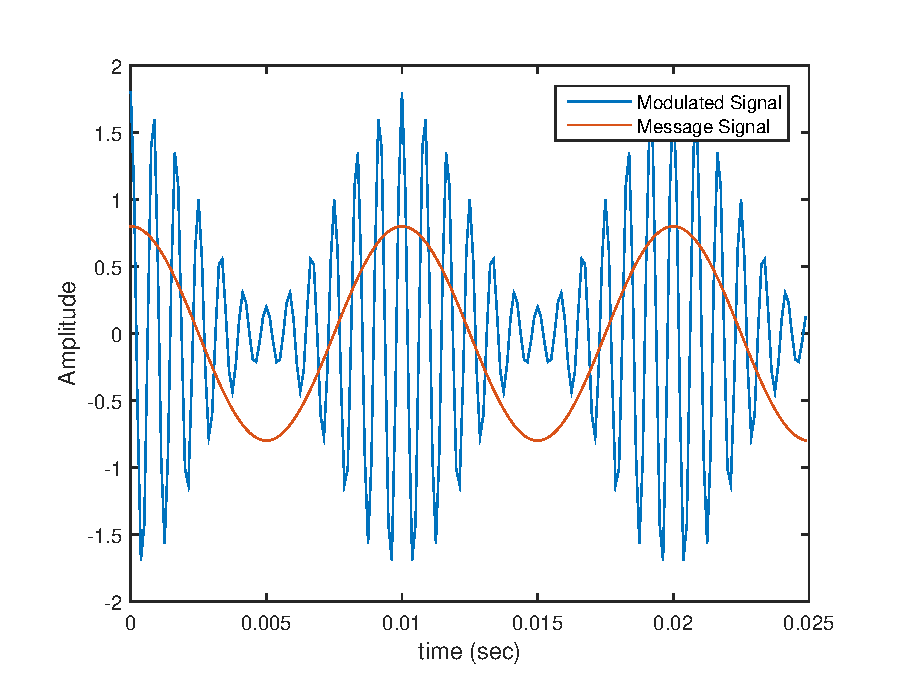
\includegraphics[scale=0.7]{fig5.eps}
	\caption{A time domain plot of the modulated signal and the original message signal.}
\end{figure}
	
\begin{figure}[H]
	\centering
	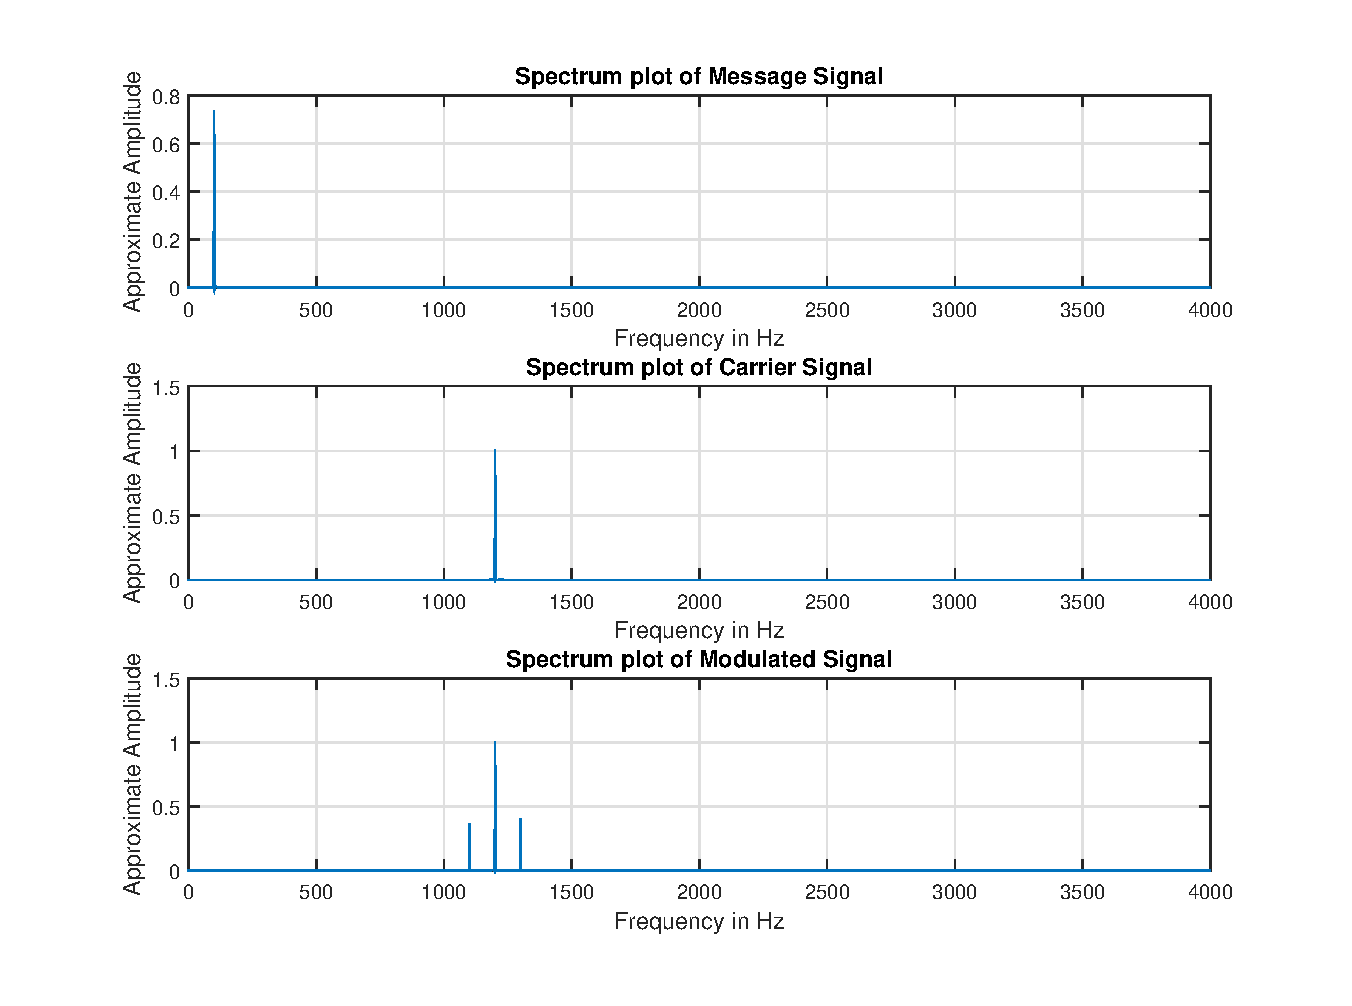
\includegraphics[scale=0.7]{fig6.eps}
	\caption{Frequency spectrograms showing the spectrum of the original message signal, the carrier signal, and the modulated signal.}
\end{figure}



\subsection{Results: AM Waveform Detection}
The demodulation of the test signal with carrier frequency 1200$\si{\hertz}$ and message signal of 100$\si{\hertz}$ was implemented in MATLAB and can be seen in Appendix F. To demodulate the test signal it was simply multiplied by the carrier signal. The multiplication of the test signal, $x(t)$, results in the following general equation:

\begin{align}
	x(t) \cdot \cos (2 \pi f_c t) = \frac{1}{2} \cdot m(t) + \frac{1}{2} + \frac{1}{2} \cdot (1 + m(t)) \cdot \cos (2 \pi (2 f_c) t)
\end{align}

Figure 8 shows the result after multiplying the test signal again by the carrier signal. We note that the original signal is now present at the 100 $\si{\hertz}$, with half its original amplitude. Additionally, there is a high frequency component of the demodulated signal that can be seen located at 2400 $\si{\hertz}$.

\begin{figure}[H]
	\begin{minipage}[t]{0.45\linewidth}
		\centering
		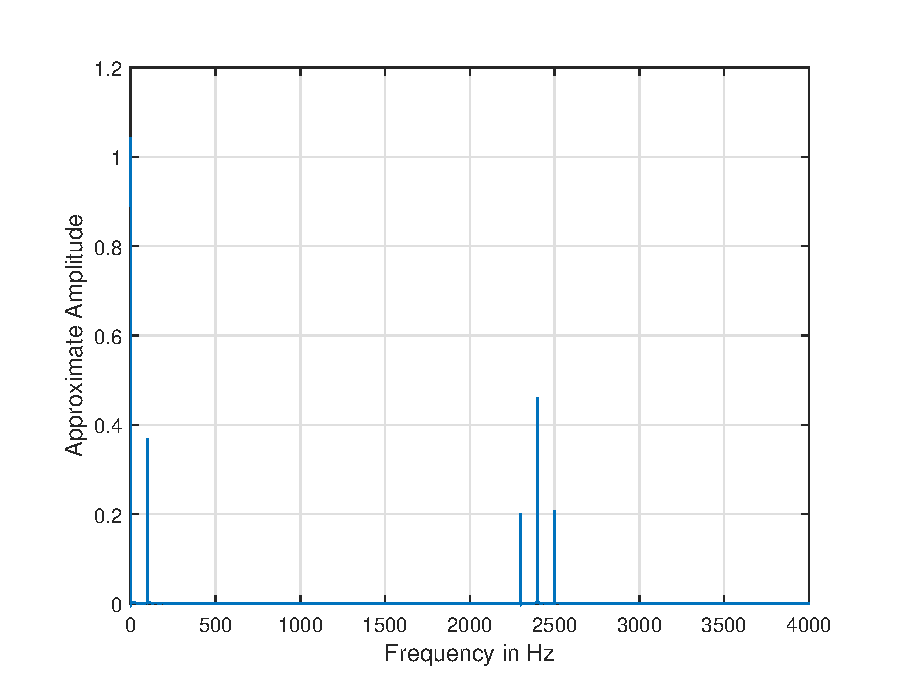
\includegraphics[scale=0.5]{fig7.eps}
		\caption{The demodulated signal. Original signal is returned at half amplitude and a higher frequency component is also \\returned.}
	\end{minipage}
	\hspace{1cm}
	\begin{minipage}[t]{0.45\linewidth}
		\centering
		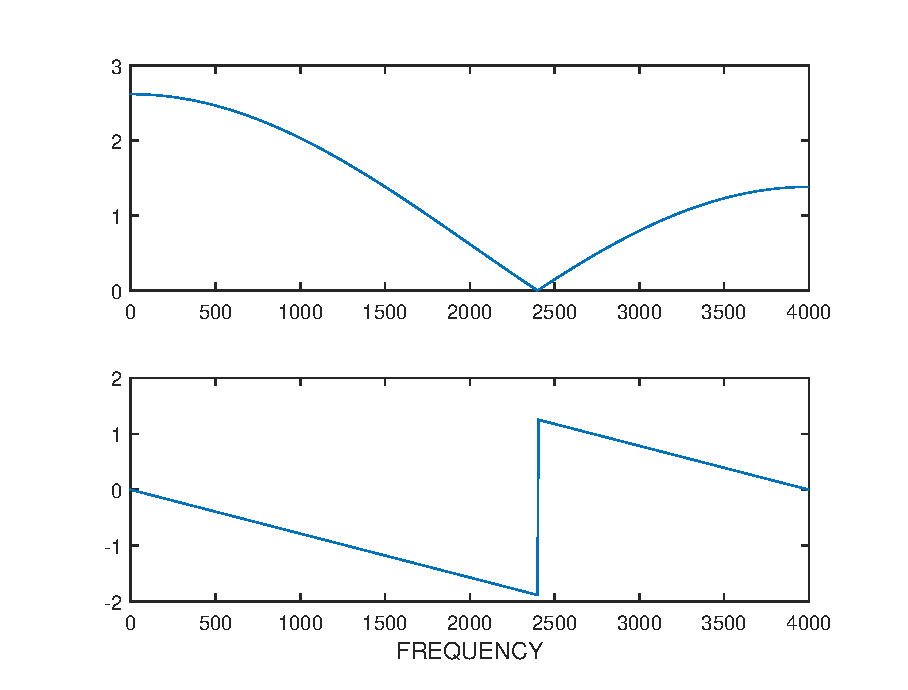
\includegraphics[scale=0.5]{fig8.eps}
		\caption{The bode plot of the three term notch filter. The top plot shows the frequency response for the amplitude of the filter. Note that a zero exists directly at the 2400 $\si{\hertz}$ frequency.}
	\end{minipage}
\end{figure}

To remove the unwanted higher frequency component from the demodulated signal, we need to use a filter. A three term notch filter was used in this instance, of the general form:
\begin{align*}
	y[n] = x[n] - 2 \cdot \cos (\hat{\omega}_{not}) \cdot x[n-1] + x[n - 2]
\end{align*}

The frequency to be removed was specified in terms of continuous time frequency, $f_{not}$. Hence, we see that $\omega_{not}$ is defined as:
\begin{align*}
	\hat{\omega}_{not} = 2 \pi \frac{f_{not}}{f_s}
\end{align*}

Given that the frequency that needs to be filtered is 2400 $\si{\hertz}$ the filter coefficients are as follows:
\begin{align*}
	b_0 = 1, \quad b_1 = -2 \cdot \cos (2 \pi (\sfrac{2400}{8000})), \quad b_2 = 1
\end{align*} 

The implementation of the filter can be seen in the MATLAB code shown in Appendix F. The frequency response of the filter can be seen in Figure 9. We note that there is a zero directly located at the 2400 $\si{\hertz}$ frequency.The filtered demodulated signal is shown in Figure 10. The plot closely resembles the original, however, it should be noted that not all of the high frequency component was filtered out - a residual amount remains which could be removed with additional filtering.\\

A second method of demodulating the signal was also implemented using MATLAB, using the pre-existing function \verb|amdemod|. The original signal, the first demodulated signal and the demodulated signal form the \verb|amdemod| function can be seen in Figure 11. The demodulation and subsequent filtering employed in the first demodulation method renders a received signal which very closely approximates the originally sent signal, which can be seen in the middle plot. The results for the second demodulation technique can be seen in the bottom plot. Daphne and Celeste (2000) describe this approximation in the following way:

\begin{center}
	\textit{U.G.L.Y. You ain't got no alibi. You ugly. Hey. Hey. You ugly.}
\end{center}

\begin{figure}[H]
	\begin{minipage}[t]{0.45\linewidth}
		\centering
		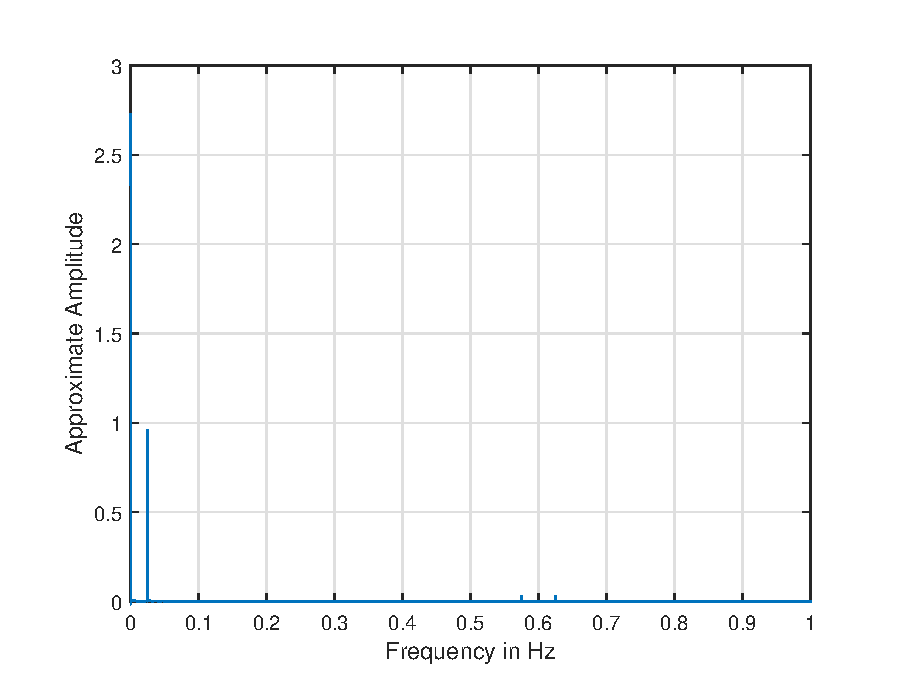
\includegraphics[scale=0.5]{fig9.eps}
		\caption{The demodulated, filtered signal - which closely resembles the original signal, $m(t)$.}
	\end{minipage}
	\hspace{1cm}
	\begin{minipage}[t]{0.45\linewidth}
		\centering
		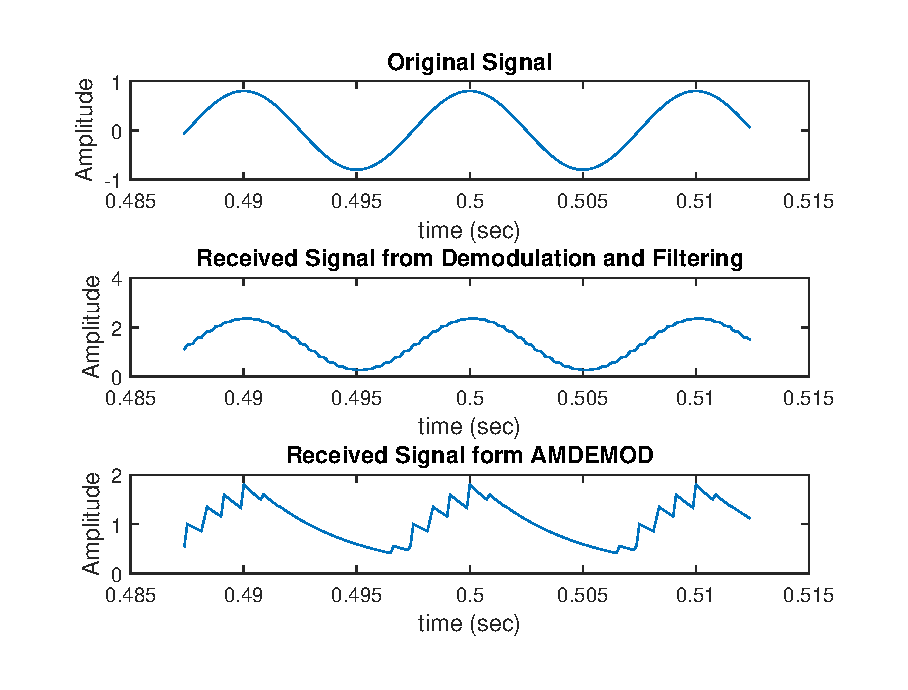
\includegraphics[scale=0.5]{fig10.eps}
		\cprotect\caption{Comparison of the original signal and the demodulated signal, using the filtering approach (middle plot) and the \verb|amdemod |function (bottom plot).}
	\end{minipage}
\end{figure}

Jokes aside, the approximation is bad using the \verb|amdemod| function. The reason for the poor approximation can be seen when looking at Figure 12. The bottom plot shows the spectrogram for the received signal using the \verb|amdemod| function, which clearly shows that there are frequency components which were not present in the original signal - this accounts for the poor approximation. The middle plot shows the spectrogram for the demodulated and filtered signal. This much cleaner, but still not perfect due to the small amount of high frequency left around the 2400 $\si{\hertz}$ from the demodulation process.

\begin{figure}[H]
	\centering
	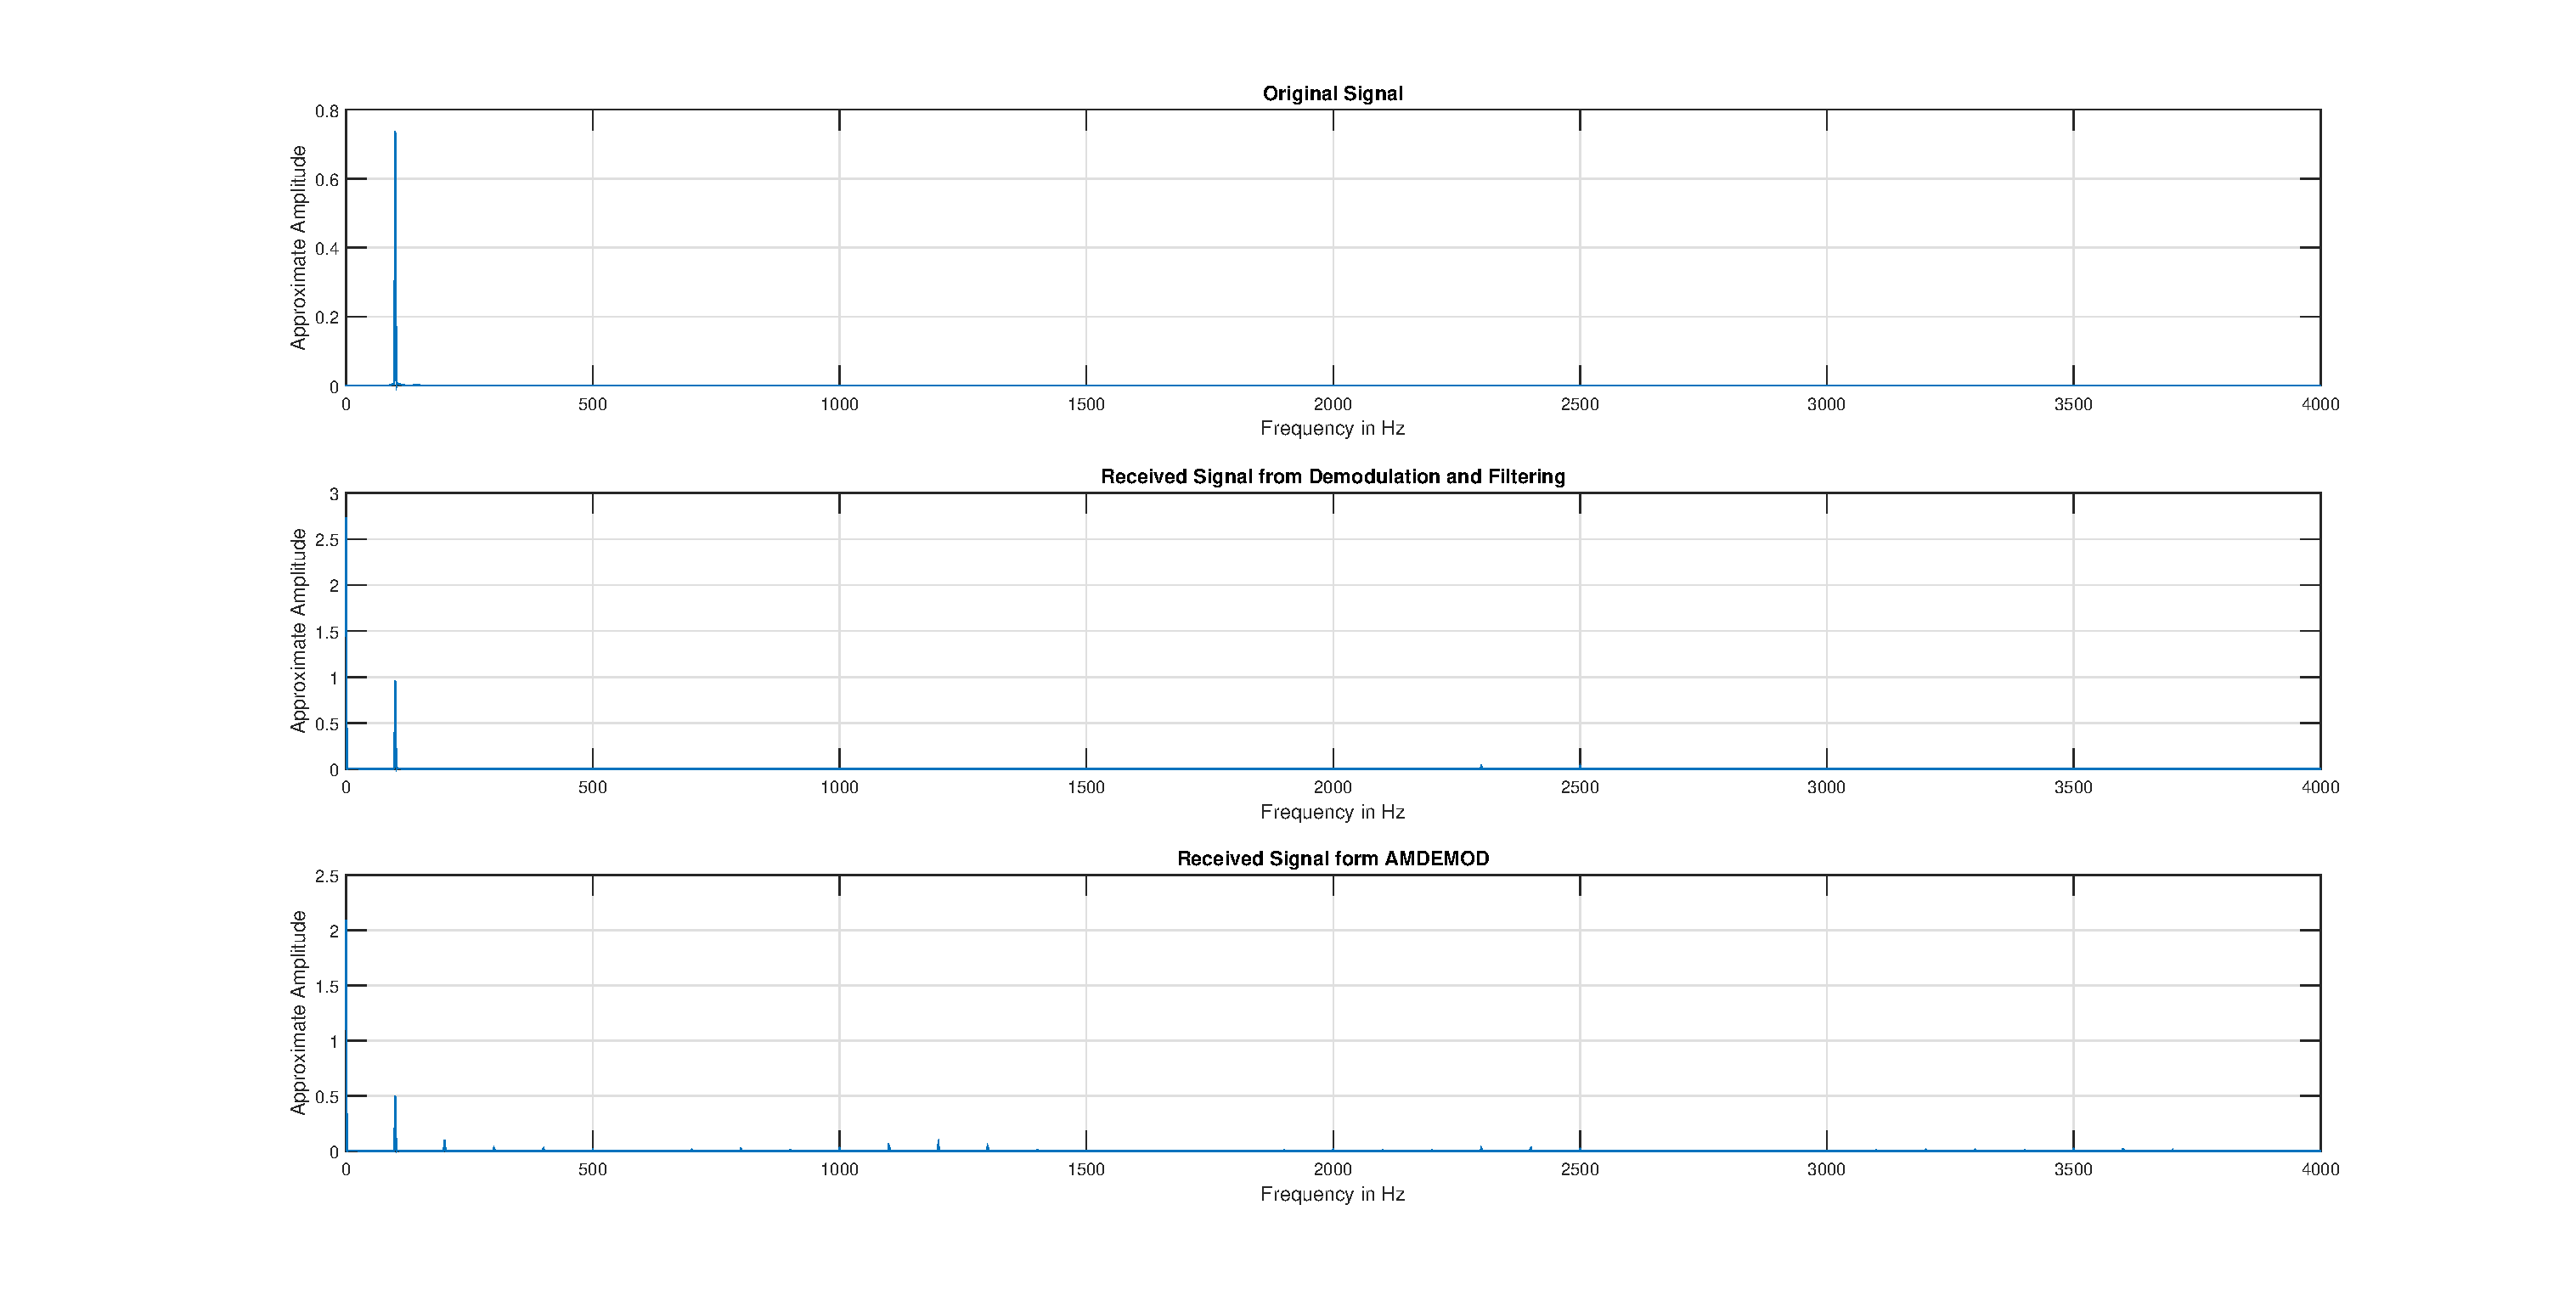
\includegraphics[scale=0.3]{fig11.eps}
	\cprotect\caption{Spectrograms of the original signal, the demodulated and filtered signal, and the signal passed to the \verb|amdemod| function, in the top, middle and bottom plots, respectively.}
\end{figure}

%----------------------------------------------------------------------------------------
%	SECTION 3
%----------------------------------------------------------------------------------------

\section{Improvements}

Improvements could be made to the demodulated and filtered signal, removing even more of the unwanted frequency components if the signal was filtered again. That is the signal would be passed through a first order filter twice. Alternatively, a second order filter could be used instead, and pass the signal through this once.

%----------------------------------------------------------------------------------------
%	BIBLIOGRAPHY
%----------------------------------------------------------------------------------------

\section{References}

Daphene, \& Celeste. (2000). \textit{We Didn't Say That}. UK: Universal\\

McClellan, J.,Schafer, R., \& Yoder, M. (2015). \textit{DSP First} (Global Edition). Harlow, England: Pearson Education Limited.

\newpage
%----------------------------------------------------------------------------------------
%	APPENDIX
%----------------------------------------------------------------------------------------

\section{Appendices}

\subsection{Appendix A}

\begin{lstlisting}
function tones = dtmfdial(nums)
% DTMFDIAL Create vector of tones which will dial a DTMF
% touch tone telephone system

% usage: tones = dtmfdial(nums)
%    nums = vector of numbers ranging from 1 to 12
%    tones = vector containing the corresponding tones

	if (nargin < 1)
		error('DTFMDIAL requires one input');
	end

	fs = 8000;   %-- This must be 8000 so dtmfdeco()will work

	freq = ([697 697 697 770 770 770 852 852 852 941 941 941;...
			1209 1336 1477 1209 1336 1477 1209 1336 1477 1209 1336 1477]);


	tone_dur = 0.5;  %-- Specify the duration of the tone
	gap_dur = 0.1;   %-- Specify the duration of the gap

	dur = (tone_dur + gap_dur)*ones(1,length(nums)); %-- Total duration

	tones = zeros(1,uint16(sum(dur)*fs + 1));    %-- Allocate memory for signal

	tt = 0:1/fs:tone_dur;    %-- Specify discrete time sample vector 
	tt_gap = length(0:1/fs:gap_dur); %-- Specify the length of gap vector
	n1 = 1;

	for i = 1:length(nums)
		% Specify frequecies for both row and col
		row_freq = freq(1,nums(i));
		col_freq = freq(2,nums(i));

		% Build a discrete time signal for tone
		tone = cos(2*pi*row_freq*tt) + cos(2*pi*col_freq*tt);

		% Build a gap for the tone
		tone_gap = zeros(1,tt_gap);

		% Add the tone to the tones vector
		n2 = n1 + length(tone) - 1;
		tones(n1:n2) = tone;
		n1 = n2;

		% Add a pause duration to the tones vector
		n2 = n1 + length(tone_gap) - 1;
		tones(n1:n2) = tone_gap;
		n1 = n2;
	end
end
\end{lstlisting}

\newpage

\subsection{Appendix B}

\begin{lstlisting}
% Clear any stored variables and the workspace
clear; clc;

L = 64; %-- length of the ????
fs = 8000; %-- set the sampling frequency

n = 0:L;
ww = 0:(pi/256):pi; %-- We only need positive frequencies

% Generate a filter h770 for the 770Hz component
h770 = (2/L)*cos((2*pi*770*n)/fs);
subplot(2,1,1)
stem(h770)
xlabel('n');
ylabel('Amplitude');
title('Filter coefficients for h770 filter')

H1 = freqz(h770,1,ww);

% Generate a filter h1336 for the 1336Hz component
h1336 = (2/L)*cos((2*pi*1336*n)/fs);
subplot(2,1,2)
stem(h1336)
xlabel('n');
ylabel('Amplitude');
title('Filter coefficients for h1336 filter')

H2 = freqz(h1336,1,ww);

ff = (ww/(2*pi))*fs;
figure(2)
plot(ff,abs(H1)); grid on;
xlabel('Frequency (Hz)')
ylabel('Amplitude')

ff = (ww/(2*pi))*fs;
figure(3)
plot(ff,abs(H2)); grid on;
xlabel('Frequency (Hz)')
ylabel('Amplitude')
\end{lstlisting}

\newpage

\subsection{Appendix C}

\begin{lstlisting}
function ss = dtmfscor(xx, freq, L, fs)
% DTMFSCOR
% ss = dtmfscor(xx, freq, L, [fs])
% returns   1 (TRUE) if freq is present
%           0 (FALSE) if freq is not present
% xx = input DTMF signal
% freq = test frequency
% L = length of FIR bandpass filter
% fs = sampling frequency (DEFAULT is 8000)
%
% The signal detectino is done by filtering xx with a length L BPF, hh,
% squaring the output, and comparing with an arbitrary setpoint based on
% the average power of xx.

	if (nargin < 4), fs = 8000; end
	nn = 0:L; %-- specify the integer set n
	hh = (2/L)*cos((2*pi*freq*nn)/fs); %-- specify the filter coefficients 
	ss = (mean(conv(xx,hh).^2) > mean(xx.^2)/5);
end
\end{lstlisting}

\hspace{1cm}

\subsection{Appendix D}

\begin{lstlisting}
function key = dtmfdeco(xx,fs)
% DTMFDECO key = dtmfdeco(xx,[fs])
% returns the key number correspoingin to the DTMF waveform, xx.
% fs = sampling freq (DEFAULT = 8000Hz if not specified)

L = 64;

if (nargin < 2), fs = 8000; end;

	tone_pairs = ...
		[697 697 697 770 770 770 852 852 852 941 941 941;
		1209 1336 1477 1209 1336 1477 1209 1336 1477 1209 1336 1477];

	for i = 1:length(tone_pairs)
		if (dtmfscor(xx, tone_pairs(1,i), L, fs) ...
				&& dtmfscor(xx, tone_pairs(2,i), L, fs))
			key = i;
			return
		end
	end
end
\end{lstlisting}

\newpage

\subsection{Appendix E}

\begin{lstlisting}
% Clear any variables and the current workspace
clear; clc;

% Set up parameters for signal generation
dur = 1; %-- Set up the signal duration
fs = 8000; %-- Set up the sampling frequency
tt = 0:1/fs:dur; %-- Set up the discrete time vector

fc = 1200;
cc = cos(2*pi*fc*tt);

fm = 100;
Am = 0.8;
mm = Am*cos(2*pi*fm*tt);

modulated_signal = (1 + mm).*cc;

figure(1)
plot(tt(1:200),modulated_signal(1:200))
hold on
plot(tt(1:200),mm(1:200))
legend('Modulated Signal','Message Signal')
xlabel('time (sec)')
ylabel('Amplitude')

figure(2)
subplot(3,1,1)
showspec(mm,fs)
title('Spectrum plot of Message Signal')
subplot(3,1,2)
showspec(cc,fs)
title('Spectrum plot of Carrier Signal')
subplot(3,1,3)
showspec(modulated_signal,fs)
title('Spectrum plot of Modulated Signal')
\end{lstlisting}

\newpage

\subsection{Appendix F}

\begin{lstlisting}
% Clear any variables and the current workspace
clear; clc;

% Set up parameters for signal generation
dur = 1; %-- Set up the signal duration
fs = 8000; %-- Set up the sampling frequency
tt = 0:1/fs:dur; %-- Set up the discrete time vector

fc = 1200;
cc = cos(2*pi*fc*tt);

fm = 100;
Am = 0.8;
mm = Am*cos(2*pi*fm*tt);

% Create modulated signal from 
modulated_signal = (1 + mm).*cc;

% Multiply the modulated signal by the carrier signal
demodulated_signal = modulated_signal.*cc;
figure(1)
showspec(demodulated_signal,fs)

% Creation of 3 term notch filter
f_notch = 2400;
w_notch = 2*pi*(f_notch/fs);
bb = [1 -2*cos(w_notch) 1];
[H,ww] = freqz(bb);
figure(2)
subplot(2,1,1)
plot(ww*fs/(2*pi),abs(H))
subplot(2,1,2)
plot(ww*fs/(2*pi),angle(H))
xlabel('NORMALIZED FREQUENCY')

yy = firfilt(bb,demodulated_signal);
figure(3)
showspec(yy)
\end{lstlisting}
%----------------------------------------------------------------------------------------


\end{document}